% Options for packages loaded elsewhere
\PassOptionsToPackage{unicode}{hyperref}
\PassOptionsToPackage{hyphens}{url}
%
\documentclass[
]{book}
\usepackage{amsmath,amssymb}
\usepackage{iftex}
\ifPDFTeX
  \usepackage[T1]{fontenc}
  \usepackage[utf8]{inputenc}
  \usepackage{textcomp} % provide euro and other symbols
\else % if luatex or xetex
  \usepackage{unicode-math} % this also loads fontspec
  \defaultfontfeatures{Scale=MatchLowercase}
  \defaultfontfeatures[\rmfamily]{Ligatures=TeX,Scale=1}
\fi
\usepackage{lmodern}
\ifPDFTeX\else
  % xetex/luatex font selection
\fi
% Use upquote if available, for straight quotes in verbatim environments
\IfFileExists{upquote.sty}{\usepackage{upquote}}{}
\IfFileExists{microtype.sty}{% use microtype if available
  \usepackage[]{microtype}
  \UseMicrotypeSet[protrusion]{basicmath} % disable protrusion for tt fonts
}{}
\makeatletter
\@ifundefined{KOMAClassName}{% if non-KOMA class
  \IfFileExists{parskip.sty}{%
    \usepackage{parskip}
  }{% else
    \setlength{\parindent}{0pt}
    \setlength{\parskip}{6pt plus 2pt minus 1pt}}
}{% if KOMA class
  \KOMAoptions{parskip=half}}
\makeatother
\usepackage{xcolor}
\usepackage{color}
\usepackage{fancyvrb}
\newcommand{\VerbBar}{|}
\newcommand{\VERB}{\Verb[commandchars=\\\{\}]}
\DefineVerbatimEnvironment{Highlighting}{Verbatim}{commandchars=\\\{\}}
% Add ',fontsize=\small' for more characters per line
\usepackage{framed}
\definecolor{shadecolor}{RGB}{248,248,248}
\newenvironment{Shaded}{\begin{snugshade}}{\end{snugshade}}
\newcommand{\AlertTok}[1]{\textcolor[rgb]{0.94,0.16,0.16}{#1}}
\newcommand{\AnnotationTok}[1]{\textcolor[rgb]{0.56,0.35,0.01}{\textbf{\textit{#1}}}}
\newcommand{\AttributeTok}[1]{\textcolor[rgb]{0.13,0.29,0.53}{#1}}
\newcommand{\BaseNTok}[1]{\textcolor[rgb]{0.00,0.00,0.81}{#1}}
\newcommand{\BuiltInTok}[1]{#1}
\newcommand{\CharTok}[1]{\textcolor[rgb]{0.31,0.60,0.02}{#1}}
\newcommand{\CommentTok}[1]{\textcolor[rgb]{0.56,0.35,0.01}{\textit{#1}}}
\newcommand{\CommentVarTok}[1]{\textcolor[rgb]{0.56,0.35,0.01}{\textbf{\textit{#1}}}}
\newcommand{\ConstantTok}[1]{\textcolor[rgb]{0.56,0.35,0.01}{#1}}
\newcommand{\ControlFlowTok}[1]{\textcolor[rgb]{0.13,0.29,0.53}{\textbf{#1}}}
\newcommand{\DataTypeTok}[1]{\textcolor[rgb]{0.13,0.29,0.53}{#1}}
\newcommand{\DecValTok}[1]{\textcolor[rgb]{0.00,0.00,0.81}{#1}}
\newcommand{\DocumentationTok}[1]{\textcolor[rgb]{0.56,0.35,0.01}{\textbf{\textit{#1}}}}
\newcommand{\ErrorTok}[1]{\textcolor[rgb]{0.64,0.00,0.00}{\textbf{#1}}}
\newcommand{\ExtensionTok}[1]{#1}
\newcommand{\FloatTok}[1]{\textcolor[rgb]{0.00,0.00,0.81}{#1}}
\newcommand{\FunctionTok}[1]{\textcolor[rgb]{0.13,0.29,0.53}{\textbf{#1}}}
\newcommand{\ImportTok}[1]{#1}
\newcommand{\InformationTok}[1]{\textcolor[rgb]{0.56,0.35,0.01}{\textbf{\textit{#1}}}}
\newcommand{\KeywordTok}[1]{\textcolor[rgb]{0.13,0.29,0.53}{\textbf{#1}}}
\newcommand{\NormalTok}[1]{#1}
\newcommand{\OperatorTok}[1]{\textcolor[rgb]{0.81,0.36,0.00}{\textbf{#1}}}
\newcommand{\OtherTok}[1]{\textcolor[rgb]{0.56,0.35,0.01}{#1}}
\newcommand{\PreprocessorTok}[1]{\textcolor[rgb]{0.56,0.35,0.01}{\textit{#1}}}
\newcommand{\RegionMarkerTok}[1]{#1}
\newcommand{\SpecialCharTok}[1]{\textcolor[rgb]{0.81,0.36,0.00}{\textbf{#1}}}
\newcommand{\SpecialStringTok}[1]{\textcolor[rgb]{0.31,0.60,0.02}{#1}}
\newcommand{\StringTok}[1]{\textcolor[rgb]{0.31,0.60,0.02}{#1}}
\newcommand{\VariableTok}[1]{\textcolor[rgb]{0.00,0.00,0.00}{#1}}
\newcommand{\VerbatimStringTok}[1]{\textcolor[rgb]{0.31,0.60,0.02}{#1}}
\newcommand{\WarningTok}[1]{\textcolor[rgb]{0.56,0.35,0.01}{\textbf{\textit{#1}}}}
\usepackage{longtable,booktabs,array}
\usepackage{calc} % for calculating minipage widths
% Correct order of tables after \paragraph or \subparagraph
\usepackage{etoolbox}
\makeatletter
\patchcmd\longtable{\par}{\if@noskipsec\mbox{}\fi\par}{}{}
\makeatother
% Allow footnotes in longtable head/foot
\IfFileExists{footnotehyper.sty}{\usepackage{footnotehyper}}{\usepackage{footnote}}
\makesavenoteenv{longtable}
\usepackage{graphicx}
\makeatletter
\def\maxwidth{\ifdim\Gin@nat@width>\linewidth\linewidth\else\Gin@nat@width\fi}
\def\maxheight{\ifdim\Gin@nat@height>\textheight\textheight\else\Gin@nat@height\fi}
\makeatother
% Scale images if necessary, so that they will not overflow the page
% margins by default, and it is still possible to overwrite the defaults
% using explicit options in \includegraphics[width, height, ...]{}
\setkeys{Gin}{width=\maxwidth,height=\maxheight,keepaspectratio}
% Set default figure placement to htbp
\makeatletter
\def\fps@figure{htbp}
\makeatother
\setlength{\emergencystretch}{3em} % prevent overfull lines
\providecommand{\tightlist}{%
  \setlength{\itemsep}{0pt}\setlength{\parskip}{0pt}}
\setcounter{secnumdepth}{5}
\usepackage{booktabs}
\ifLuaTeX
  \usepackage{selnolig}  % disable illegal ligatures
\fi
\usepackage[]{natbib}
\bibliographystyle{plainnat}
\IfFileExists{bookmark.sty}{\usepackage{bookmark}}{\usepackage{hyperref}}
\IfFileExists{xurl.sty}{\usepackage{xurl}}{} % add URL line breaks if available
\urlstyle{same}
\hypersetup{
  pdftitle={Comunidad para el Desarrollo},
  pdfauthor={Renzo Álvarez Carcheri},
  hidelinks,
  pdfcreator={LaTeX via pandoc}}

\title{Comunidad para el Desarrollo}
\usepackage{etoolbox}
\makeatletter
\providecommand{\subtitle}[1]{% add subtitle to \maketitle
  \apptocmd{\@title}{\par {\large #1 \par}}{}{}
}
\makeatother
\subtitle{Análisis de datos con STATA: aplicaciones con encuestas}
\author{Renzo Álvarez Carcheri}
\date{2023-12-28}

\usepackage{amsthm}
\newtheorem{theorem}{Theorem}[chapter]
\newtheorem{lemma}{Lemma}[chapter]
\newtheorem{corollary}{Corollary}[chapter]
\newtheorem{proposition}{Proposition}[chapter]
\newtheorem{conjecture}{Conjecture}[chapter]
\theoremstyle{definition}
\newtheorem{definition}{Definition}[chapter]
\theoremstyle{definition}
\newtheorem{example}{Example}[chapter]
\theoremstyle{definition}
\newtheorem{exercise}{Exercise}[chapter]
\theoremstyle{definition}
\newtheorem{hypothesis}{Hypothesis}[chapter]
\theoremstyle{remark}
\newtheorem*{remark}{Remark}
\newtheorem*{solution}{Solution}
\begin{document}
\maketitle

{
\setcounter{tocdepth}{1}
\tableofcontents
}
\hypertarget{introducciuxf3n}{%
\chapter{Introducción}\label{introducciuxf3n}}

This is a \emph{sample} book written in \textbf{Markdown}. You can use anything that Pandoc's Markdown supports; for example, a math equation \(a^2 + b^2 = c^2\).

\hypertarget{usos}{%
\section{Usos}\label{usos}}

Each \textbf{bookdown} chapter is an .Rmd file, and each .Rmd file can contain one (and only one) chapter. A chapter \emph{must} start with a first-level heading: \texttt{\#\ A\ good\ chapter}, and can contain one (and only one) first-level heading.

Use second-level and higher headings within chapters like: \texttt{\#\#\ A\ short\ section} or \texttt{\#\#\#\ An\ even\ shorter\ section}.

The \texttt{index.Rmd} file is required, and is also your first book chapter. It will be the homepage when you render the book.

\hypertarget{instalaciuxf3n}{%
\section{Instalación}\label{instalaciuxf3n}}

You can render the HTML version of this example book without changing anything:

\begin{enumerate}
\def\labelenumi{\arabic{enumi}.}
\item
  Find the \textbf{Build} pane in the RStudio IDE, and
\item
  Click on \textbf{Build Book}, then select your output format, or select ``All formats'' if you'd like to use multiple formats from the same book source files.
\end{enumerate}

Or build the book from the R console:

\begin{Shaded}
\begin{Highlighting}[]
\NormalTok{bookdown}\SpecialCharTok{::}\FunctionTok{render\_book}\NormalTok{()}
\end{Highlighting}
\end{Shaded}

To render this example to PDF as a \texttt{bookdown::pdf\_book}, you'll need to install XeLaTeX. You are recommended to install TinyTeX (which includes XeLaTeX): \url{https://yihui.org/tinytex/}.

\hypertarget{entorno}{%
\section{Entorno}\label{entorno}}

As you work, you may start a local server to live preview this HTML book. This preview will update as you edit the book when you save individual .Rmd files. You can start the server in a work session by using the RStudio add-in ``Preview book'', or from the R console:

\begin{Shaded}
\begin{Highlighting}[]
\NormalTok{bookdown}\SpecialCharTok{::}\FunctionTok{serve\_book}\NormalTok{()}
\end{Highlighting}
\end{Shaded}

\hypertarget{recomendaciones}{%
\section{Recomendaciones}\label{recomendaciones}}

\hypertarget{aspectos-buxe1sicos}{%
\chapter{Aspectos básicos}\label{aspectos-buxe1sicos}}

All chapters start with a first-level heading followed by your chapter title, like the line above. There should be only one first-level heading (\texttt{\#}) per .Rmd file.

\hypertarget{uso-del-do-file-editor}{%
\section{Uso del do-file editor}\label{uso-del-do-file-editor}}

\hypertarget{uso-del-comando-help}{%
\section{Uso del comando Help}\label{uso-del-comando-help}}

\hypertarget{empezando-a-programar}{%
\chapter{Empezando a programar}\label{empezando-a-programar}}

\hypertarget{carga-y-anuxe1lisis-descriptivo-de-datos}{%
\section{Carga y análisis descriptivo de datos}\label{carga-y-anuxe1lisis-descriptivo-de-datos}}

En Stata podemos cargar datos internos y externos. Los primeros podemos llamarlos a través del comando \texttt{help\ dta\_examples}. Al ejecutar este comando, veremos que dispondremos de más de 25 conjuntos de datos los cuales podemos llamar usando el comando \texttt{sysuse}. Para los datos externos de formato .dta usaremos el comando \texttt{use}, mientras que para otros formatos como .csv, .xls, .xlsx, .dbf, entre otros; se usará el comando \texttt{import}.

\hypertarget{datos-internos}{%
\subsection{Datos internos}\label{datos-internos}}

Para este ejemplo, usaremos el conjunto de datos interno ``auto'' seguido de la opción \texttt{clear} ya que nos permite limpiar la memoria de cualquier otro dataset usado previamente. Seguido de ello, usaremos el comando \texttt{describe} para que Stata nos brinde una descripción general de dicho dataset.

\begin{Shaded}
\begin{Highlighting}[]
\KeywordTok{sysuse}\NormalTok{ auto, }\KeywordTok{clear}
\KeywordTok{describe}
\end{Highlighting}
\end{Shaded}

\begin{verbatim}
(1978 Automobile Data)


Contains data from D:\OneDrive - Superintendencia Nacional de Servicios de Sane
> amiento\Escritorio\Stata16\ado\base/a/auto.dta
  obs:            74                          1978 Automobile Data
 vars:            12                          13 Apr 2018 17:45
                                              (_dta has notes)
-------------------------------------------------------------------------------
              storage   display    value
variable name   type    format     label      variable label
-------------------------------------------------------------------------------
make            str18   %-18s                 Make and Model
price           int     %8.0gc                Price
mpg             int     %8.0g                 Mileage (mpg)
rep78           int     %8.0g                 Repair Record 1978
headroom        float   %6.1f                 Headroom (in.)
trunk           int     %8.0g                 Trunk space (cu. ft.)
weight          int     %8.0gc                Weight (lbs.)
length          int     %8.0g                 Length (in.)
turn            int     %8.0g                 Turn Circle (ft.)
displacement    int     %8.0g                 Displacement (cu. in.)
gear_ratio      float   %6.2f                 Gear Ratio
foreign         byte    %8.0g      origin     Car type
-------------------------------------------------------------------------------
Sorted by: foreign
\end{verbatim}

Inmediatamente Stata nos informa que la data esta relacionada con datos asociados a automóviles del año 1978, la cual exhibe 74 observaciones con 12 variables que, al hacer una lectura rápida de la columna de etiquetas de la variable (variable label), están vinculadas a las características físicas de los vehículos tales como: el peso (weight) y el largo (length), así como el espacio de la maletera (trunk) y el espacio libre (headroom). Asimismo, existen variables asociadas al precio (price), millas recorridas por galón (mpg), entre otras. Finalmente, es importante resaltar que de las 12 variables, 11 de ellas son de tipo numérico y solo 1 de tipo texto o cadena.

Para seguir conociendo este dataset, ahora usaremos el comando \texttt{summarize} con la finalidad de que Stata nos muestre los principales estadísticos descriptivos de la data.

\begin{Shaded}
\begin{Highlighting}[]
\KeywordTok{summarize}
\end{Highlighting}
\end{Shaded}

\begin{verbatim}
(1978 Automobile Data)

    Variable |        Obs        Mean    Std. Dev.       Min        Max
-------------+---------------------------------------------------------
        make |          0
       price |         74    6165.257    2949.496       3291      15906
         mpg |         74     21.2973    5.785503         12         41
       rep78 |         69    3.405797    .9899323          1          5
    headroom |         74    2.993243    .8459948        1.5          5
-------------+---------------------------------------------------------
       trunk |         74    13.75676    4.277404          5         23
      weight |         74    3019.459    777.1936       1760       4840
      length |         74    187.9324    22.26634        142        233
        turn |         74    39.64865    4.399354         31         51
displacement |         74    197.2973    91.83722         79        425
-------------+---------------------------------------------------------
  gear_ratio |         74    3.014865    .4562871       2.19       3.89
     foreign |         74    .2972973    .4601885          0          1
\end{verbatim}

La tabla nos muestra estadísticos descriptivos básicos como la media, desviación estándar y los valores mínimos y máximos. Como se observa, estos estadísticos son aplicables solo a variables numéricas, por esa razón el contenido de la tabla para la variable marca (make) esta vacía. Asimismo, podemos utilizar la opción del comando \texttt{summarize} denominado \texttt{detail} para obtener información estadística adicional como la varianza, el sesgo y la kurtosis, así como una serie de percentiles que nos permitirán realizar un análisis descriptivo más detallado. Empleemos este comando con la variable precio (price):

\begin{Shaded}
\begin{Highlighting}[]
\KeywordTok{summarize}\NormalTok{ price, }\KeywordTok{detail}
\end{Highlighting}
\end{Shaded}

\begin{verbatim}
(1978 Automobile Data)

                            Price
-------------------------------------------------------------
      Percentiles      Smallest
 1%         3291           3291
 5%         3748           3299
10%         3895           3667       Obs                  74
25%         4195           3748       Sum of Wgt.          74

50%       5006.5                      Mean           6165.257
                        Largest       Std. Dev.      2949.496
75%         6342          13466
90%        11385          13594       Variance        8699526
95%        13466          14500       Skewness       1.653434
99%        15906          15906       Kurtosis       4.819188
\end{verbatim}

Otro comando que usaremos frecuentemente es el comando \texttt{codebook} ya que nos permitirá obtener información complementaria a la antes vista, esta vez sin importar si la variable es número o texto. Utilicemos este comando para la variable de tipo texto llamada marca (make).

\begin{Shaded}
\begin{Highlighting}[]
\KeywordTok{codebook}\NormalTok{ make}
\end{Highlighting}
\end{Shaded}

\begin{verbatim}
(1978 Automobile Data)


-------------------------------------------------------------------------------
make                                                             Make and Model
-------------------------------------------------------------------------------

                  type:  string (str18), but longest is str17

         unique values:  74                       missing "":  0/74

              examples:  "Cad. Deville"
                         "Dodge Magnum"
                         "Merc. XR-7"
                         "Pont. Catalina"

               warning:  variable has embedded blanks
\end{verbatim}

Como acabamos de ver, el comando \texttt{codebook} nos muestra información muy importante para cualquier analista de datos, en particular, sobre los valores únicos (unique values) y valores pérdidos (missing values). En este caso, Stata nos señala que la variable marca (make) tiene 74 valores único y 0/74 missings values. Esto último significa que los autos de la muestra los componen 74 autos de marcas diferentes, de los cuales para el 100\% de la muestra se encuentra dicha información.

\hypertarget{datos-externos}{%
\subsection{Datos externos}\label{datos-externos}}

Stata puede importar sin ningún problema datos en formato .dta; para cuáles son las posibilidades que tenemos para importar archivos debemos escribir el comando \texttt{help\ import}. La ventana que muestra el Stata permite observar todos los formatos compatibles a importar, por lo que solo bastaría tener claridad de que tipo de formato queremos importar para acceder a la sintaxis y empezar a cargar nuestros datos. Aquí un ejemplo para importar archivos de formato excel.

\begin{Shaded}
\begin{Highlighting}[]
\NormalTok{import excel }\StringTok{"ruta del archivo.xlsx"}\NormalTok{, firstrow sheet(}\StringTok{"Sheet1"}\NormalTok{) }\KeywordTok{clear}
\end{Highlighting}
\end{Shaded}

En el término ``ruta del archivo.xlsx'' del código debemos ingresar la ruta en la cual tenemos nuestro archivo .xlsx que deseamos importar al Stata. Por su parte, la opción ``firstrow'' señala al Stata que la primera fila de nuestro archivo excel debe ser considerada como la lista de variables. Finalmente, ``sheet()'' es una opción para especificar la hoja del libro excel, lo que es sumamente importante cuando manejamos varias hojas dentro de un mismo libro.

Una vez importado el archivo, podemos iniciar nuestro análisis descriptivo que vimos en la sección anterior.

\hypertarget{tipo-de-variables-y-formatos}{%
\section{Tipo de variables y formatos}\label{tipo-de-variables-y-formatos}}

Profundicemos un poco sobre las variables y formatos ya que son parte fundamental en la gestión de datos. Afortunadamente, en Stata trabajaremos con solo variables de clase númerica y texto por lo que no será muy complejo abordar esta sección.

\hypertarget{tipos-de-almacenamiento}{%
\subsection{Tipos de almacenamiento}\label{tipos-de-almacenamiento}}

Las variables numéricas y textos se almacenarán en la memoria a través de diferentes tipologías. Comenzando por las variables numéricas tenemos los siguientes tipos de almacenamiento: byte, int, long, float y double.

Cada tipología esta directamente relacionado con su tamaño de almacenamiento en términos de ``bytes''. Así, una variable númerica de tipo ``byte'' tendrá un peso de 1 ``bytes'' en la memoria, de modo que este tipo de variable estará usualmente asociada con números de hasta 3 caracteres.

Podemos obtener ayuda del Stata para conocer las distintas tipologías de variables que se manejan. Así, al escribir el comando \texttt{help\ Data\ types} podemos observar todas las tipologías tanto para las variables numéricas y texto, las cuales siguen la misma lógica del párrafo anterior.

En cuanto a los formatos, estos son aplicables a las variables numéricas y nos permitirán generar una visualización personalizada de dichas variables. La manera de acceder a toda la caja de formatos será escribiendo el siguiente comando: \texttt{help\ format}.

Es importante señalar que para Stata no es imprescindible que especifiquemos el tipo de almacenamiento y los formatos ya que el Stata establece las establece por defecto. De hecho, podemos gestionar las variables de un dataset sin siquiera colocar alguna línea referida al tipo de almacenamiento y su formato. Por ejemplo, al utilizar el comando \texttt{generate\ edad\ =\ 10} estamos creando una nueva variable para un determinado dataset, esta variable tomará el nombre de ``edad'' y tendrá como valores el número 10. En este caso, no estamos señalandole al Stata explícitamente el tipo de almacenamiento que tendrá esta variable y aún así Stata lo creará. Ahora bien, si revisamos a través del comando \texttt{codebook\ edad} nos mostrará que el tipo de almacenamiento definido por defecto por el Stata es ``float''. Sin embargo, por los valores que aborda esta variable ``edad'' es totalmente factible que la variable sea de tipo ``byte'' en lugar de ``float'', de manera tal que podemos ahorrarnos algunos bytes en la memoria sin perjudicar la calidad de los datos.

\hypertarget{cross}{%
\chapter{Explorando la ENAHO}\label{cross}}

Cross-references make it easier for your readers to find and link to elements in your book.

\hypertarget{uso-de-encuestas-en-el-anuxe1lisis-de-datos}{%
\section{Uso de encuestas en el análisis de datos}\label{uso-de-encuestas-en-el-anuxe1lisis-de-datos}}

There are two steps to cross-reference any heading:

\begin{enumerate}
\def\labelenumi{\arabic{enumi}.}
\tightlist
\item
  Label the heading: \texttt{\#\ Hello\ world\ \{\#nice-label\}}.

  \begin{itemize}
  \tightlist
  \item
    Leave the label off if you like the automated heading generated based on your heading title: for example, \texttt{\#\ Hello\ world} = \texttt{\#\ Hello\ world\ \{\#hello-world\}}.
  \item
    To label an un-numbered heading, use: \texttt{\#\ Hello\ world\ \{-\#nice-label\}} or \texttt{\{\#\ Hello\ world\ .unnumbered\}}.
  \end{itemize}
\item
  Next, reference the labeled heading anywhere in the text using \texttt{\textbackslash{}@ref(nice-label)}; for example, please see Chapter \ref{cross}.

  \begin{itemize}
  \tightlist
  \item
    If you prefer text as the link instead of a numbered reference use: \protect\hyperlink{cross}{any text you want can go here}.
  \end{itemize}
\end{enumerate}

\hypertarget{caracteruxedsticas-de-la-enaho}{%
\section{Características de la ENAHO}\label{caracteruxedsticas-de-la-enaho}}

Figures and tables \emph{with captions} can also be cross-referenced from elsewhere in your book using \texttt{\textbackslash{}@ref(fig:chunk-label)} and \texttt{\textbackslash{}@ref(tab:chunk-label)}, respectively.

See Figure \ref{fig:nice-fig}.

\begin{Shaded}
\begin{Highlighting}[]
\FunctionTok{par}\NormalTok{(}\AttributeTok{mar =} \FunctionTok{c}\NormalTok{(}\DecValTok{4}\NormalTok{, }\DecValTok{4}\NormalTok{, .}\DecValTok{1}\NormalTok{, .}\DecValTok{1}\NormalTok{))}
\FunctionTok{plot}\NormalTok{(pressure, }\AttributeTok{type =} \StringTok{\textquotesingle{}b\textquotesingle{}}\NormalTok{, }\AttributeTok{pch =} \DecValTok{19}\NormalTok{)}
\end{Highlighting}
\end{Shaded}

\begin{figure}

{\centering 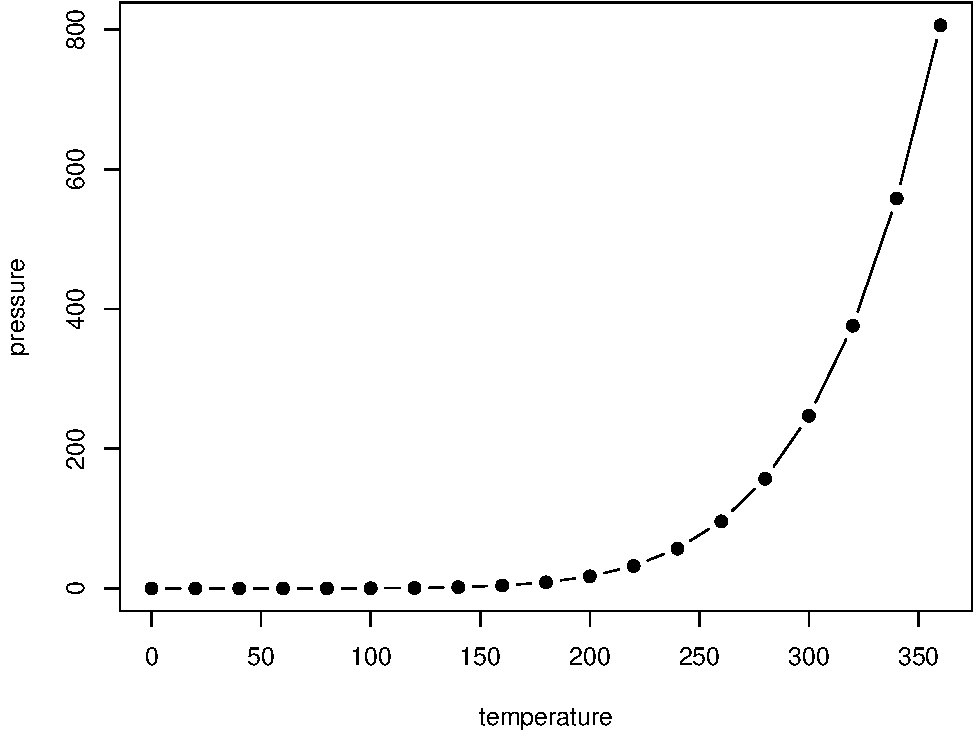
\includegraphics[width=0.8\linewidth]{_main_files/figure-latex/nice-fig-1} 

}

\caption{Here is a nice figure!}\label{fig:nice-fig}
\end{figure}

Don't miss Table \ref{tab:nice-tab}.

\begin{Shaded}
\begin{Highlighting}[]
\NormalTok{knitr}\SpecialCharTok{::}\FunctionTok{kable}\NormalTok{(}
  \FunctionTok{head}\NormalTok{(pressure, }\DecValTok{10}\NormalTok{), }\AttributeTok{caption =} \StringTok{\textquotesingle{}Here is a nice table!\textquotesingle{}}\NormalTok{,}
  \AttributeTok{booktabs =} \ConstantTok{TRUE}
\NormalTok{)}
\end{Highlighting}
\end{Shaded}

\begin{table}

\caption{\label{tab:nice-tab}Here is a nice table!}
\centering
\begin{tabular}[t]{rr}
\toprule
temperature & pressure\\
\midrule
0 & 0.0002\\
20 & 0.0012\\
40 & 0.0060\\
60 & 0.0300\\
80 & 0.0900\\
\addlinespace
100 & 0.2700\\
120 & 0.7500\\
140 & 1.8500\\
160 & 4.2000\\
180 & 8.8000\\
\bottomrule
\end{tabular}
\end{table}

\hypertarget{descripciuxf3n-inicial-de-los-datos}{%
\section{Descripción inicial de los datos}\label{descripciuxf3n-inicial-de-los-datos}}

\hypertarget{gestiuxf3n-de-datos-con-enaho}{%
\chapter{Gestión de datos con ENAHO}\label{gestiuxf3n-de-datos-con-enaho}}

You can add parts to organize one or more book chapters together. Parts can be inserted at the top of an .Rmd file, before the first-level chapter heading in that same file.

Add a numbered part: \texttt{\#\ (PART)\ Act\ one\ \{-\}} (followed by \texttt{\#\ A\ chapter})

Add an unnumbered part: \texttt{\#\ (PART\textbackslash{}*)\ Act\ one\ \{-\}} (followed by \texttt{\#\ A\ chapter})

Add an appendix as a special kind of un-numbered part: \texttt{\#\ (APPENDIX)\ Other\ stuff\ \{-\}} (followed by \texttt{\#\ A\ chapter}). Chapters in an appendix are prepended with letters instead of numbers.

\hypertarget{gestiuxf3n-del-muxf3dulo-100}{%
\section{Gestión del módulo 100}\label{gestiuxf3n-del-muxf3dulo-100}}

El módulo 100 corresponde al módulo de las ``Características de la Vivienda y del Hogar'' por lo que inmediatamente iniciamos la programación abriendo el archivo formato .dta denominado ``enaho01-2022-100''.

\begin{Shaded}
\begin{Highlighting}[]
\NormalTok{cd }\StringTok{"ruta del archivo"}
\KeywordTok{use}\NormalTok{ enaho01{-}2022{-}100, }\KeywordTok{clear}
\end{Highlighting}
\end{Shaded}

Ahora bien, empezaremos con las variables identificadoras; estas son las variables conglome, vivienda y hogar las cuales describiremos a continuación:

\begin{Shaded}
\begin{Highlighting}[]
\KeywordTok{describe}\NormalTok{ conglome vivienda hogar}
\end{Highlighting}
\end{Shaded}

\begin{verbatim}
> itorio\renzo\asesorías\Noemy\data\enaho01-2022-100.dta", clear

              storage   display    value
variable name   type    format     label      variable label
-------------------------------------------------------------------------------
conglome        str6    %6s                   numero de conglomerado
vivienda        str3    %3s                   numero de seleccion de vivienda
hogar           str2    %2s                   numero secuencial del hogar
\end{verbatim}

El resultado anterior nos muestra que las variables identificadoras son de tipo texto, de 2 a 6 caracteres, que refieren al número de conglomerado, número de selección de la vivienda y número secuencial del hogar. Finalmente, empleados un \texttt{codebook} para observar lo valores únicos y los missings values.

\begin{Shaded}
\begin{Highlighting}[]
\KeywordTok{codebook}\NormalTok{ conglome vivienda hogar}
\end{Highlighting}
\end{Shaded}

\begin{verbatim}
> torio\renzo\asesorías\Noemy\data"
D:\OneDrive - Superintendencia Nacional de Servicios de Saneamiento\Escritorio\
> renzo\asesorías\Noemy\data



-------------------------------------------------------------------------------
conglome                                                 numero de conglomerado
-------------------------------------------------------------------------------

                  type:  string (str6)

         unique values:  5,359                    missing "":  0/44,122

              examples:  "015258"
                         "016496"
                         "017790"
                         "019115"

-------------------------------------------------------------------------------
vivienda                                        numero de seleccion de vivienda
-------------------------------------------------------------------------------

                  type:  string (str3)

         unique values:  649                      missing "":  0/44,122

              examples:  "024"
                         "052"
                         "081"
                         "120"

-------------------------------------------------------------------------------
hogar                                               numero secuencial del hogar
-------------------------------------------------------------------------------

                  type:  string (str2)

         unique values:  15                       missing "":  0/44,122

              examples:  "11"
                         "11"
                         "11"
                         "11"
\end{verbatim}

Como observamos, los tres identificadores están presentes para las 44,122 observaciones lo que sugiere que todos las viviendas se encuentran identificadas. Asimismo, existen 5,359 valores únicos de conglomerados; esto nos indica que las 44,122 viviendas de la muestra han sido seleccionadas de tal modo que pertecen a alguno de los 5,359 conglomerados, 649 viviendas y cuentan con algún número secuencial del hogar asignado.

En tal sentido, las variables ``conglome'', ``vivienda'' y ``hogar'' serán una suerte de ``documento de identidad'' que nos permitirá individualizar a las viviendas. Con la finalidad de efectuar esto último, usamos la función \texttt{group()} del comando \texttt{egen}, en la que crearemos una variable denominada ``id''.

\begin{Shaded}
\begin{Highlighting}[]
\KeywordTok{egen}\NormalTok{ id = }\FunctionTok{group}\NormalTok{(conglome vivienda hogar)}
\end{Highlighting}
\end{Shaded}

Luego, corroboramos que esta variable se encuentre dispersa en toda la muestra y que, además, sean valores únicos, por lo que usaremos las funciones \texttt{count}.

\begin{Shaded}
\begin{Highlighting}[]
\FunctionTok{count} \KeywordTok{if}\NormalTok{ id}
\end{Highlighting}
\end{Shaded}

\begin{verbatim}
> torio\renzo\asesorías\Noemy\data"
D:\OneDrive - Superintendencia Nacional de Servicios de Saneamiento\Escritorio\
> renzo\asesorías\Noemy\data



  44,122
\end{verbatim}

\hypertarget{gestiuxf3n-del-muxf3dulo-200}{%
\section{Gestión del módulo 200}\label{gestiuxf3n-del-muxf3dulo-200}}

\hypertarget{gestiuxf3n-del-muxf3dulo-300}{%
\section{Gestión del módulo 300}\label{gestiuxf3n-del-muxf3dulo-300}}

\hypertarget{gestiuxf3n-del-muxf3dulo-400}{%
\section{Gestión del módulo 400}\label{gestiuxf3n-del-muxf3dulo-400}}

\hypertarget{gestiuxf3n-del-muxf3dulo-500}{%
\section{Gestión del módulo 500}\label{gestiuxf3n-del-muxf3dulo-500}}

\hypertarget{integrando-muxf3dulos}{%
\section{Integrando módulos}\label{integrando-muxf3dulos}}

\hypertarget{anuxe1lisis-inferencial}{%
\chapter{Análisis inferencial}\label{anuxe1lisis-inferencial}}

\hypertarget{revisiuxf3n-del-modelos-de-regresiuxf3n}{%
\section{Revisión del modelos de regresión}\label{revisiuxf3n-del-modelos-de-regresiuxf3n}}

Footnotes are put inside the square brackets after a caret \texttt{\^{}{[}{]}}. Like this one \footnote{This is a footnote.}.

\hypertarget{principales-comandos-para-regresiones}{%
\section{Principales comandos para regresiones}\label{principales-comandos-para-regresiones}}

Reference items in your bibliography file(s) using \texttt{@key}.

For example, we are using the \textbf{bookdown} package \citep{R-bookdown} (check out the last code chunk in index.Rmd to see how this citation key was added) in this sample book, which was built on top of R Markdown and \textbf{knitr} \citep{xie2015} (this citation was added manually in an external file book.bib).
Note that the \texttt{.bib} files need to be listed in the index.Rmd with the YAML \texttt{bibliography} key.

The RStudio Visual Markdown Editor can also make it easier to insert citations: \url{https://rstudio.github.io/visual-markdown-editing/\#/citations}

\hypertarget{inferencias-con-factores-de-expansiuxf3n}{%
\section{Inferencias con factores de expansión}\label{inferencias-con-factores-de-expansiuxf3n}}

\hypertarget{aplicaciuxf3n-con-encuestas}{%
\section{Aplicación con encuestas}\label{aplicaciuxf3n-con-encuestas}}

\hypertarget{gestiuxf3n-con-datos-de-panel-enaho}{%
\chapter{Gestión con datos de panel ENAHO}\label{gestiuxf3n-con-datos-de-panel-enaho}}

\hypertarget{aspectos-a-tener-en-cuenta}{%
\section{Aspectos a tener en cuenta}\label{aspectos-a-tener-en-cuenta}}

Here is an equation.

\begin{equation} 
  f\left(k\right) = \binom{n}{k} p^k\left(1-p\right)^{n-k}
  \label{eq:binom}
\end{equation}

You may refer to using \texttt{\textbackslash{}@ref(eq:binom)}, like see Equation \eqref{eq:binom}.

\hypertarget{comandos-para-panel-de-datos}{%
\section{Comandos para panel de datos}\label{comandos-para-panel-de-datos}}

Labeled theorems can be referenced in text using \texttt{\textbackslash{}@ref(thm:tri)}, for example, check out this smart theorem \ref{thm:tri}.

\begin{theorem}
\protect\hypertarget{thm:tri}{}\label{thm:tri}For a right triangle, if \(c\) denotes the \emph{length} of the hypotenuse
and \(a\) and \(b\) denote the lengths of the \textbf{other} two sides, we have
\[a^2 + b^2 = c^2\]
\end{theorem}

Read more here \url{https://bookdown.org/yihui/bookdown/markdown-extensions-by-bookdown.html}.

\hypertarget{aplicaciuxf3n-economuxe9trica}{%
\section{Aplicación econométrica}\label{aplicaciuxf3n-economuxe9trica}}

The R Markdown Cookbook provides more help on how to use custom blocks to design your own callouts: \url{https://bookdown.org/yihui/rmarkdown-cookbook/custom-blocks.html}

\hypertarget{extra}{%
\chapter{Extra}\label{extra}}

\hypertarget{uso-de-globals-y-locals}{%
\section{Uso de globals y locals}\label{uso-de-globals-y-locals}}

HTML books can be published online, see: \url{https://bookdown.org/yihui/bookdown/publishing.html}

\hypertarget{uso-de-comandos-forvalue-y-foreach}{%
\section{Uso de comandos forvalue y foreach}\label{uso-de-comandos-forvalue-y-foreach}}

By default, users will be directed to a 404 page if they try to access a webpage that cannot be found. If you'd like to customize your 404 page instead of using the default, you may add either a \texttt{\_404.Rmd} or \texttt{\_404.md} file to your project root and use code and/or Markdown syntax.

\hypertarget{almacenamiento-y-reporte-de-resultados}{%
\section{Almacenamiento y reporte de resultados}\label{almacenamiento-y-reporte-de-resultados}}

Bookdown HTML books will provide HTML metadata for social sharing on platforms like Twitter, Facebook, and LinkedIn, using information you provide in the \texttt{index.Rmd} YAML. To setup, set the \texttt{url} for your book and the path to your \texttt{cover-image} file. Your book's \texttt{title} and \texttt{description} are also used.

This \texttt{gitbook} uses the same social sharing data across all chapters in your book- all links shared will look the same.

Specify your book's source repository on GitHub using the \texttt{edit} key under the configuration options in the \texttt{\_output.yml} file, which allows users to suggest an edit by linking to a chapter's source file.

Read more about the features of this output format here:

\url{https://pkgs.rstudio.com/bookdown/reference/gitbook.html}

Or use:

\begin{Shaded}
\begin{Highlighting}[]
\NormalTok{?bookdown}\SpecialCharTok{::}\NormalTok{gitbook}
\end{Highlighting}
\end{Shaded}


  \bibliography{book.bib,packages.bib}

\end{document}
